\subsection{EZ-PICARD}

% add image here
\begin{figure}[ht]
    \centering
    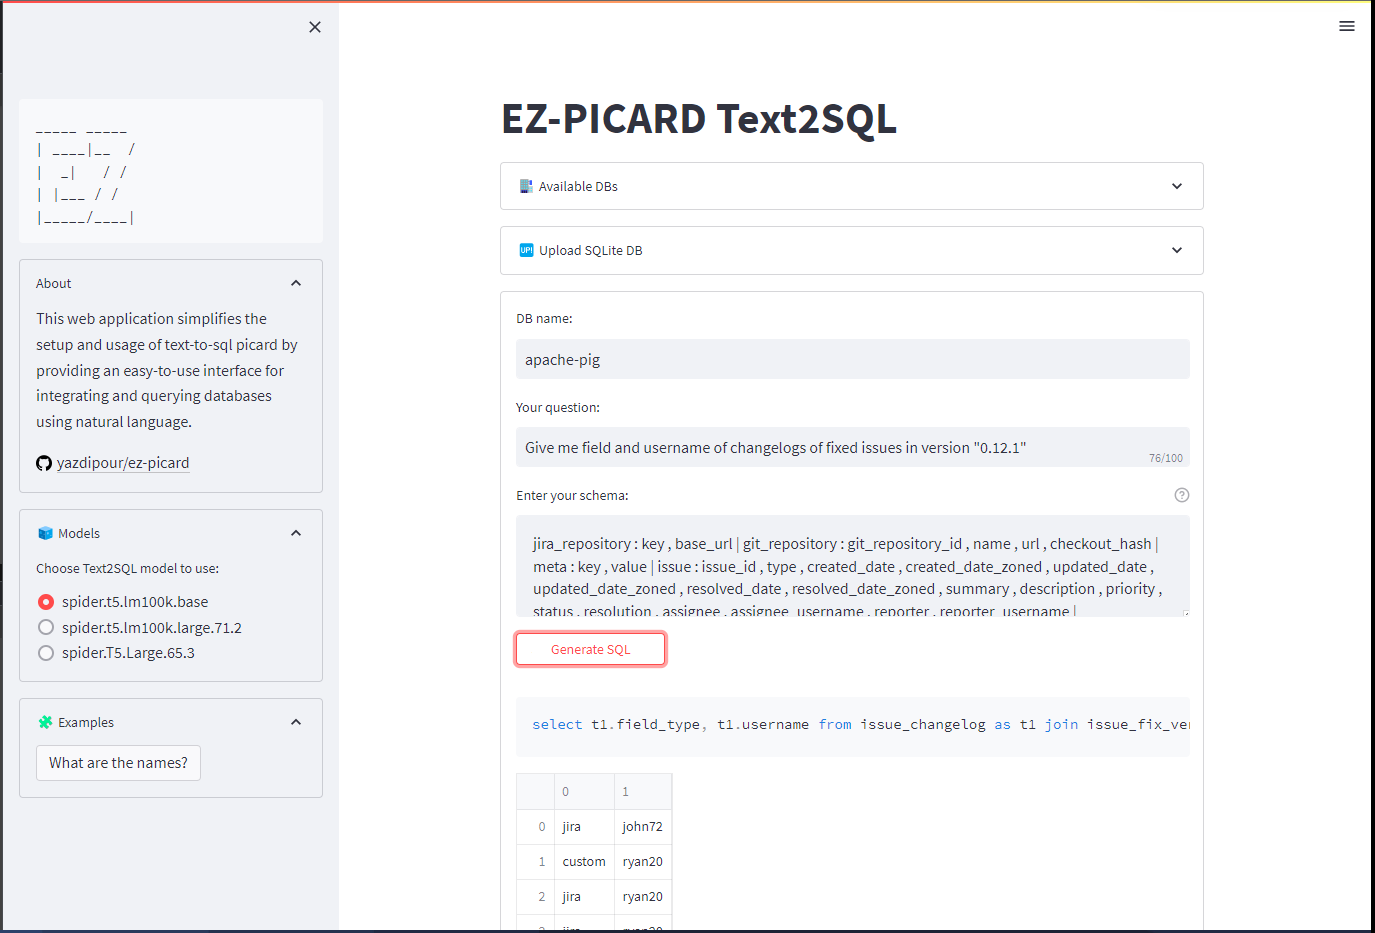
\includegraphics[width=1\textwidth]{pics/ez/ui.png}
    \caption{EZ-PICARD Web Application}
    \label{fig:ezpicard}
\end{figure}

\subsubsection{Microservices Practices}

% add image here
\begin{figure}[ht]
    \centering
    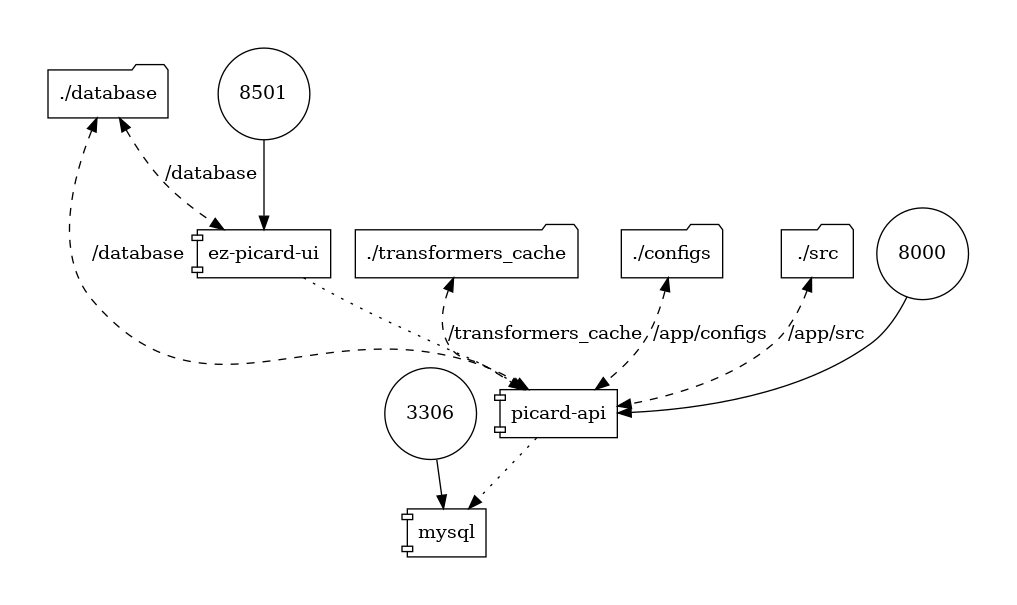
\includegraphics[width=0.8\textwidth]{pics/ez/map.png}
    \caption{EZ-PICARD Architecture}
\end{figure}


\subsubsection{DB Engines}

The Picard Method is a method for constrained inference on top of an existing model, but it is not a model itself. Currently, the PICARD parser and the supporting software are not supported for PostgreSQL, MySQL and others, which would require changes to the PICARD parser, translation of Spider databases and text-to-SQL data, and retraining models to produce MSSQL code. To use the Picard Method, a complex toolchain of Haskell code is built with CABAL and requires a complicated toolchain for the Facebook Thrift library.

After the setup, the Picard server can be started by running the compiled standalone executable PICARD. This executable is responsible for providing the necessary information to the user, such as specific parameters and options within the constrained inference. It is important to note that the Picard Method is not a full-fledged model; therefore, it is necessary to combine it with an existing model to get a complete inference system.

The thrift library is used for communication between the parser and the beam search algorithm. The parser, written in the efficient and powerful Haskell programming language, is used in combination with the hf transformers, which is a Python package. To further expand the scope of the system, new SQL engines can be supported by adding a parser for each one.

These parsers also need to be written in Haskell, as the existing SQLite parser is of limited use in this regard, as it has been written to work best on Spider's subset of SQLite and only supports part of the SQLite specification. This means that more advanced parsers must be created to maximize the system's capabilities. Additionally, these parsers need to be written with a high level of precision in order to ensure that the system can effectively communicate with various engines and databases.